\chapter{Desenvolvimento}
\label{cap:desenvolvimento}

\section{Infraestrutura de Experimentação e Coleta de Métricas}
\label{sec:infra_experimental}

Para comparar as metodologias de forma precisa, é necessário configurar o ambiente para que os testes sejam feitos em cima das mesmas condições. Nesse sentido, antes de comparar as métricas, foi construída uma infraestrutura de automação, responsável por subir as aplicações, gerar a carga e coletar as métricas. Essa infraestrutura concentra os procedimentos de execução e de coleta em um único conjunto de scripts, de modo que para realizar um novo teste, não é necessário refazer manualmente o processo.

Com base nisso, as medições foram realizadas em um único ambiente fixo: Windows 11, processador AMD Ryzen 7 5700X3D, 32 GB de memória, Docker Engine 29.7.2 e Docker Compose v5.4.0. Manter o ambiente permite comparar tempos de construção e perfis de consumo de recursos entre snapshots. Também, foram adotadas regras de isolamento, como manter os recursos atribuídos ao Docker constantes e encerrar contêineres externos ao experimento antes de cada medição, para não afetar a amostragem de processamento e de memória nem a contagem de componentes.

A execução de cada aplicação se apoia em contêineres Docker orquestrados por \texttt{docker compose}. Cada aplicação sobe com seus serviços de apoio, como banco de dados e, quando aplicável, cache e proxy reverso. Para que a referência base das aplicações iniciais e decomposições partam do mesmo estado, um script de \emph{seed} determinístico popula o banco com um conjunto equivalente de dados de demonstração. As portas são fixadas por aplicação, conforme uma tabela de portas própria para o experimento, de modo a evitar colisões e preservar a reprodutibilidade.

A coleta cobre oito métricas, distribuídas nas quatro categorias de medição definidas no Capítulo \ref{cap:metodologia}: tempo de construção da imagem, tempo de inicialização, consumo de processamento e de memória em repouso e sob carga, tamanho das imagens, vazão máxima e percentis de latência sob carga, Linhas de Código, contagem de componentes físicos e violações de fronteiras lógicas. A carga sintética é gerada com a ferramenta \emph{autocannon}. A contagem de Linhas de Código e as violações de fronteiras lógicas vêm de análise estática.

Cada métrica é amostrada três vezes, e o conjunto de resultados brutos e processados é armazenado por aplicação, metodologia e snapshot. As tabelas e figuras apresentadas neste capítulo são geradas automaticamente a partir desses arquivos, o que mantém a rastreabilidade entre a medição e os valores apresentados.

\section{Arquitetura de Referência}
\label{sec:arquitetura_referencia}

Nessa seção, é apresentada a arquitetura base das aplicações utilizadas na pesquisa. Com base nisso, avaliam-se os módulos, fronteiras e interações entre as partes de cada sistema, de modo que seja possível identificar os pontos de emprego de cada uma das metodologias sem ferir o funcionamento e o fluxo das aplicações.

\subsection*{Sistema de Inventário}

\begin{figure}[htb]
\caption{Diagrama de componentes do sistema de inventário (Snapshot 0).}
\label{fig:inventario_arquitetura}
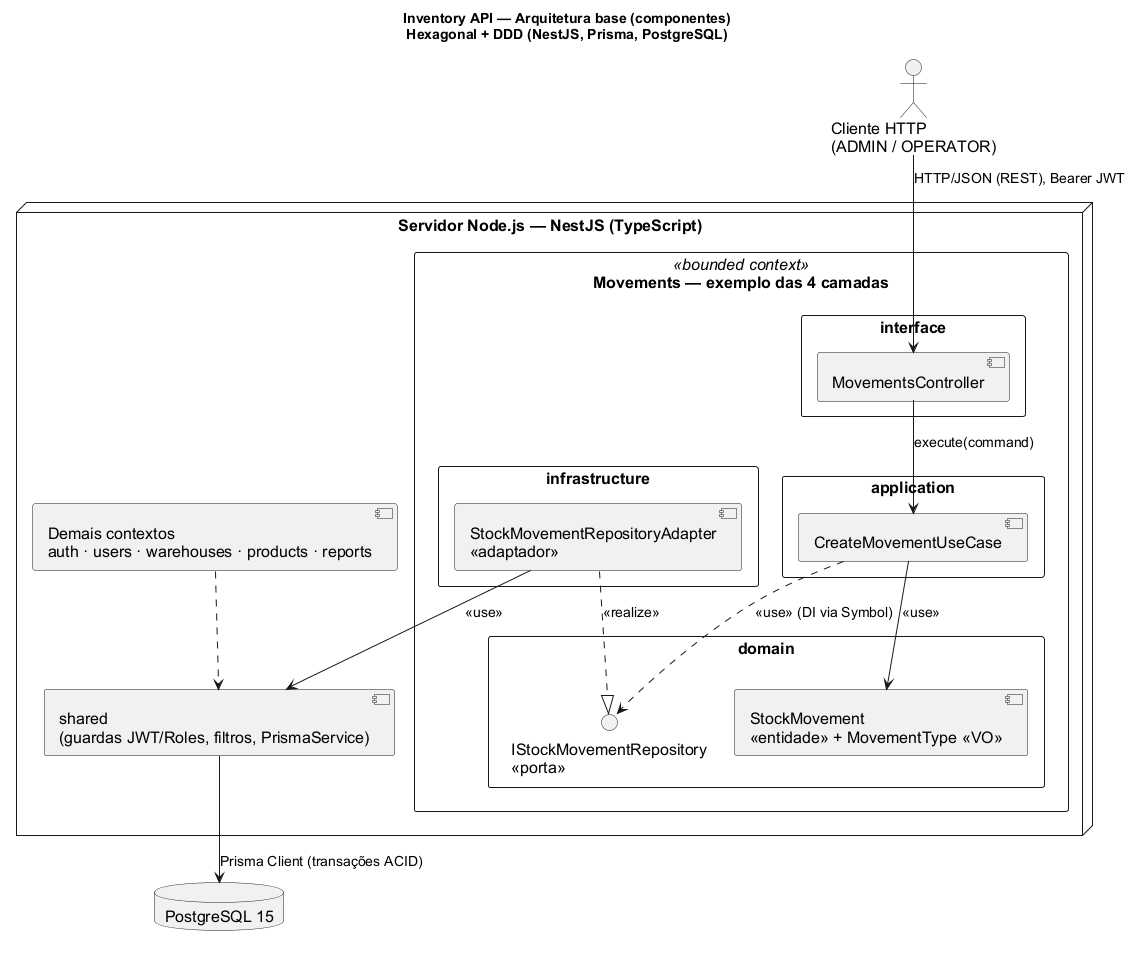
\includegraphics[width=\textwidth]{figuras/inventario__arquitetura.png}
\legend{Fonte: elaborado pelo autor (2026).}
\end{figure}

O sistema de inventário é um monólito modular desenvolvido em NestJS (TypeScript), no qual cada contexto delimitado do domínio ocupa um módulo próprio, conforme o ADR-0002. A organização interna segue a arquitetura hexagonal: cada módulo é dividido em quatro camadas --- interface, aplicação, domínio e infraestrutura. A camada de interface expõe os controladores HTTP; a de aplicação orquestra os casos de uso; a de domínio concentra as entidades, os objetos de valor e as portas; e a de infraestrutura implementa essas portas com os adaptadores. As dependências apontam de fora para dentro: a interface conhece a aplicação, que conhece o domínio, enquanto a infraestrutura depende das interfaces de porta definidas pelo domínio. Essa inversão de dependência mantém o domínio isolado dos frameworks e do banco, o que permite extrair um módulo como serviço sem reescrever suas regras.

A Figura \ref{fig:inventario_arquitetura} detalha o módulo \texttt{movements} como representante dessa estrutura. O \texttt{MovementsController} recebe a requisição e aciona o \texttt{CreateMovementUseCase}; o caso de uso opera sobre a entidade \texttt{StockMovement} e o objeto de valor \texttt{MovementType} e depende da porta \texttt{IStockMovementRepository}, não de uma implementação concreta. O \texttt{StockMovementRepositoryAdapter}, na infraestrutura, realiza essa porta e acessa o banco. É nesse módulo que está a regra central do sistema: o estoque é calculado como a soma das entradas menos a das saídas, e a escrita exige transação atômica para impedir retiradas acima do disponível (ADR-0006 e ADR-0008). Os demais contextos --- \texttt{auth}, \texttt{users}, \texttt{warehouses}, \texttt{products} e \texttt{reports} --- seguem a mesma estrutura de quatro camadas e aparecem resumidos no diagrama.

Duas responsabilidades são comuns a todos os módulos e ficam concentradas no núcleo transversal \texttt{shared}: as guardas de autenticação e papéis (\texttt{JwtAuthGuard} e \texttt{RolesGuard}), os filtros e interceptores que padronizam erros e respostas, e o \texttt{PrismaService}, que encapsula o acesso ao banco. A persistência é feita em um único PostgreSQL, acessado por meio do Prisma, com transações atômicas nos casos de escrita. Os contextos dependem desse núcleo, mas não entre si, de modo que as fronteiras lógicas permanecem isoladas.

Na borda, o sistema expõe uma única interface REST sob \texttt{/api}, protegida por token JWT e papéis. O acesso é feito por um cliente HTTP com dois perfis, \texttt{ADMIN} e \texttt{OPERATOR}, que compartilham as mesmas rotas com permissões distintas. Essa arquitetura serve de referência comum às três metodologias, pois os seis contextos e suas quatro camadas formam o ponto de partida idêntico para cada decomposição.

\subsection*{Sistema de Leilões}

\subsection*{E-commerce}

\section{Decomposição por Capacidade de Negócio}
\label{sec:metodologia_capacidade}

\subsection*{Sistema de Inventário}

\subsection*{Sistema de Leilões}

\subsection*{E-commerce}

\section{Decomposição por Subdomínio (DDD)}
\label{sec:metodologia_subdominio}

\subsection*{Sistema de Inventário}

\subsection*{Sistema de Leilões}

\subsection*{E-commerce}

\section{Decomposição por Transações}
\label{sec:metodologia_transacoes}

\subsection*{Sistema de Inventário}

\subsection*{Sistema de Leilões}

\subsection*{E-commerce}

\section{Comparação entre as Metodologias}
\label{sec:comparacao_metodologias}

\section{Síntese do Capítulo}
\label{sec:sintese_capitulo}
